\documentclass{sig-alternate}
\usepackage[utf8]{inputenc}
\usepackage{times}
\usepackage{gensymb}
\usepackage{epsfig}
\usepackage{xcolor}
\usepackage{xspace}
\usepackage{multicol}
\usepackage{listings}
\usepackage{verbatim}
\usepackage{hyperref}
\usepackage{caption}
\usepackage{subcaption}
\usepackage{float}

\usepackage[protrusion=true,expansion=true]{microtype}
\setlength{\emergencystretch}{3em}

\lstset{
basicstyle=\ttfamily\scriptsize,       % the size of the fonts that are used for the code
numbers=left,                   % where to put the line-numbers
numberstyle=\ttfamily,      % the size of the fonts that are used for the line-numbers
%aboveskip=0pt,
%belowskip=0pt,
stepnumber=1,                   % the step between two line-numbers. If it is 1 each line will be numbered
%numbersep=10pt,                  % how far the line-numbers are from the code
breakindent=0pt,
firstnumber=1,
%backgroundcolor=\color{white},  % choose the background color. You must add \usepackage{color}
showspaces=false,               % show spaces adding particular underscores
showstringspaces=false,         % underline spaces within strings
showtabs=false,                 % show tabs within strings adding particular underscores
frame=leftline,
tabsize=2,  		% sets default tabsize to 2 spaces
captionpos=b,   		% sets the caption-position to bottom
breaklines=true,    	% sets automatic line breaking
breakatwhitespace=true,    % sets if automatic breaks should only happen at whitespace
columns=fixed,
basewidth=0.52em,
xleftmargin=6mm,
xrightmargin=-6mm,
numberblanklines=false,
language=Java,
morekeywords={table,scratch,channel,interface,periodic,bloom,state,bootstrap,morph,monotone,lset,lbool,lmax,lmap},
escapeinside={(*}{*)}
}


\begin{document}
\conferenceinfo{CIDR '17}{January 8-11, 2017, Chaminade, CA, USA}
\newcommand{\smallitem}[1]{\vspace{0.5em}\noindent\textbf{#1}}
\newcommand{\smallitembot}{\vspace{0.5em}\noindent}
\bibliographystyle{abbrv}

\newcommand{\jmh}[1]{{\textcolor{red}{[[#1 -- jmh]]}}}
\newcommand{\joey}[1]{{\textcolor{cyan}{[[#1 -- jeg]]}}}
\newcommand{\msd}[1]{{\textcolor{green}{[[#1 -- msd]]}}}
\newcommand{\akon}[1]{{\textcolor{orange}{[[#1 -- akon]]}}}
\newcommand{\vikram}[1]{{\textcolor{blue}{[[#1 --vikram]]}}}
% \newcommand{\jmh}[1]{}
% \newcommand{\joey}[1]{}
% \newcommand{\msd}[1]{}
% \newcommand{\akon}[1]{}
% \newcommand{\vikram}[1]{}

% \newcommand{\cab}{CAB\xspace}
\newcommand{\versiongraph}{version graph\xspace}
\newcommand{\modelgraph}{model graph\xspace}
\newcommand{\lineagegraph}{lineage graph\xspace}
\newcommand{\VersionGraph}{Version Graph\xspace}
\newcommand{\ModelGraph}{Model Graph\xspace}
\newcommand{\LineageGraph}{Lineage Graph\xspace}

\newcommand{\version}{\kw{Version}\xspace}
\newcommand{\richversion}{\kw{RichVersion}\xspace}
\newcommand{\itemground}{\kw{Item}\xspace}
\newcommand{\GroundItem}{\kw{Item}\xspace}
\newcommand{\node}{\kw{Node}\xspace}
\newcommand{\edge}{\kw{Edge}\xspace}
\newcommand{\structure}{\kw{Structure}\xspace}
\newcommand{\graph}{\kw{Graph}\xspace}
\newcommand{\TVID}{\kw{TVID}\xspace}
\newcommand{\gtag}{\kw{Tag}\xspace}
\newcommand{\uri}{\kw{URI}\xspace}

% \newcommand{\versiongraph}{versiongraph\xspace}
% \newcommand{\modelgraph}{modelgraph\xspace}
% \newcommand{\lineagegraph}{lineagegraph\xspace}
% \newcommand{\versiongraphs}{versiongraphs\xspace}
% \newcommand{\modelgraphs}{modelgraphs\xspace}
% \newcommand{\lineagegraphs}{lineagegraphs\xspace}
\newcommand{\groundwire}{GroundWire\xspace}

\newcommand{\kw}[1]{{\small\texttt{#1}}}
\newcommand{\lilemail}[1]{\email{\small #1}}



\title{Establishing Common Ground with Data Context}

\numberofauthors{1}
\author{
\alignauthor
Joseph M.\ Hellerstein\textsuperscript{*}\textsuperscript{$\degree$}, 
Vikram Sreekanti\textsuperscript{*}, 
Joseph E. Gonzalez\textsuperscript{*},
James Dalton\textsuperscript{$\triangle$},
Akon Dey\textsuperscript{$\sharp$}, 
Sreyashi Nag\textsuperscript{$\S$}, 
Krishna Ramachandran\textsuperscript{$\natural$}, 
Sudhanshu Arora\textsuperscript{$\ddagger$},
Arka Bhattacharyya\textsuperscript{*},
Shirshanka Das\textsuperscript{$\dagger$}, 
Mark Donsky\textsuperscript{$\ddagger$}, 
Gabriel Fierro\textsuperscript{*},
Chang She\textsuperscript{$\ddagger$},
Eric Sun\textsuperscript{$\dagger$}, 
Carl Steinbach\textsuperscript{$\dagger$}
Venkat Subramanian\textsuperscript{$\flat$}\\
{\small
\textsuperscript{*}UC Berkeley,
\textsuperscript{$\degree$}Trifacta,
\textsuperscript{$\triangle$}Capital One,
\textsuperscript{$\sharp$}Awake Networks,
\textsuperscript{$\S$}University of Delhi,
\textsuperscript{$\natural$}Skyhigh Networks,
\textsuperscript{$\ddagger$}Cloudera,
\textsuperscript{$\dagger$}LinkedIn,
\textsuperscript{$\flat$}Dataguise
}
}

\maketitle

\begin{abstract}
\emph{Ground} is an open-source \emph{data context service}, a system to manage all the peripheral information that informs the use of data. 
Data usage has changed both philosophically and practically in the last decade, creating an opportunity for new data context services to foster further innovation.
In this paper we frame the challenges of managing data context along three axes: \emph{Applications}, \emph{Behavior}, and \emph{Change}. 
We provide motivation and design guidelines, present our initial design of a common metamodel and API, and explore the current state of the storage solutions that could serve the needs of a data context service. 
Throughout, we highlight opportunities for new research and engineering solutions.
\end{abstract}

\section{From Crisis to Opportunity}
Traditional database management systems were developed in an era of risk-averse design.
The technology itself was expensive, as was the on-site cost of managing it. Expertise
was scarce and concentrated in a handful of computing and consulting firms.

Two conservative design patterns emerged that lasted many decades. First, the accepted best practices
for deploying databases revolved around tight control of schemas and data ingest in support of 
general-purpose accounting and compliance use cases. 
Typical advice from data
warehousing leaders held that 
\emph{``There is no point in 
bringing data $\ldots$ into the data warehouse environment without integrating it''}~\cite{inmon2005building}. 
Second, 
the data management systems designed for these users were often built by a single vendor and deployed as a
monolithic stack. 
A traditional DBMS included a consistent storage engine, a dataflow engine, 
a language compiler and optimizer, a runtime scheduler, a metadata catalog, and facilities for data ingest 
and queueing---all designed to work closely together.


As computing and data have become orders of magnitude more efficient, changes have emerged for both of these patterns. 
Usage is changing profoundly, as expertise and control shifts from the central accountancy of an IT department to 
the domain expertise of ``business units'' tasked with extracting value from data~\cite{gartner}. 
The changes in economics and usage brought on the ``three Vs'' of Big Data: Volume, Velocity and Variety.
Resulting best practices focus on open-ended schema-on-use
data ``lakes'' and agile development, in support of exploratory analytics and innovative application intelligence~\cite{patil2012data}. 
Second, while many pieces of systems software that have emerged in this space are familiar, the overriding architecture is profoundly 
different. In today's leading open source
data management stacks, nearly all of the components 
of a traditional DBMS are explicitly independent 
and interchangeable.  This architectural decoupling is 
a critical and under-appreciated aspect of the Big Data movement,
% swappable, with multiple choices in wide use today. 
enabling more rapid innovation and specialization.

\subsection{Crisis: Big Metadata}

An unfortunate consequence of the disaggregated nature of contemporary data systems
is the lack of a standard mechanism
to assemble a collective understanding of the origin, scope, and usage of the data they manage.
In the absence of a better solution to this pressing need, the 
Hive Metastore is sometimes used, but it only serves simple relational schemas---a dead end for representing a Variety of data. 
As a result, data lake projects typically lack 
even the most rudimentary information about the data they contain or how it is being used. 
For emerging Big Data customers and vendors, this \emph{Big Metadata} problem is hitting a crisis point.  

Two significant classes of end-user problems follow directly from the absence of shared metadata services.
The first is poor productivity.
Analysts are often unable to discover what data exists, much less how it has been previously used by peers. 
Valuable data is left unused
and human effort is routinely duplicated---particularly in a schema-on-use world with raw data that requires preparation.  
``Tribal knowledge'' is a common description for how organizations manage this productivity problem. 
This is clearly not a systematic solution, and scales very poorly as organizations grow.

The second problem 
stemming from the absence of a system to track metadata 
is governance risk. 
Data management necessarily entails tracking or controlling who accesses data, what they do with it, where they put it, and how it gets consumed downstream. 
%In some cases this governance metadata is used to enforce policy (e.g.\ access control for Personally Identifiable Information); in others it is logged to support audits for compliance (e.g.\ in the Basel Committee on Banking Supervision). 
In the absence of a standard place to store metadata and answer these questions, it is impossible to enforce policies and/or audit behavior. 
As a result, many administrators marginalize their Big Data stack as a playpen for non-critical data, and thereby inhibit both the adoption and the potential of new technologies.

% In our diverse experiences in industry, the authors 
% \joey{I think we should drop this paragraph.  This paragraph is only our personal assessment of our credibility which is hard to trust.}\jmh{I dunno, the reason we have so many people on this paper is because we've seen this problem in the field. Thoughts on how to word it differently but make that point?}\joey{Fine! it's not a bad paragraph and if we keep the big author list its compelling.}

In our experiences deploying and managing systems in production, we 
have seen the need for a common service layer to support the capture, publishing and sharing of metadata information in a flexible way. 
The effort in this paper began by addressing that need.

\subsection{Opportunity: Data Context}
\jmh{would be nice to weave agility in more aggressively}
The lack of metadata services in the Big Data stack can be viewed as an opportunity:
% is both a modern crisis
% but also an 
% clean-slate 
a clean slate to rethink how we track and leverage modern usage of data.
Storage economics and schema-on-use agility suggest that the Data Lake movement could go much farther than Data Warehousing in enabling diverse, widely-used central repositories of data that can adapt to new data formats and rapidly changing organizations.
In that spirit, we advocate rethinking traditional metadata in a far more comprehensive sense. 
More generally, what we should strive to capture is the full context of data.

To emphasize the conceptual shifts of this \emph{data context}, and as a complement to the ``three Vs'' of Big Data,
we introduce three key sources of information---the \textbf{ABCs of Data Context}. Each represents a major change from the simple metadata of traditional enterprise data management.

\smallitem{Applications}: Application context is the core information that describes how raw bits get interpreted for use. 
In modern agile scenarios, application context is often relativistic (many schemas for the same data) and complex (with custom code for data interpretation). 
Application context ranges from basic data descriptions (encodings, schemas, ontologies, tags), to statistical models and parameters, to user annotations.  
All of the artifacts involved---transformation scripts, view definitions, model parameters, training sets, etc.---are critical aspects of application context. 

\smallitem{Behavior}: This is information about how data was created and used over time. 
In decoupled systems, behavioral context spans multiple services, applications and formats and often originates from high-volume sources (e.g., machine-generated usage logs).
Not only must we track upstream lineage---
the data sets and code that led to the creation of the data object---but we must also track the 
downstream lineage, including the data products that were derived from this data object. 
Aside from data lineage, behavioral context includes logs of usage: the ``digital exhaust'' left behind by computations on the data. 
As a result, behavioral context metadata can 
often be larger than the data itself. 

\smallitem{Change}:
This is information about the version history of data and associated code, including changes over time to both structure and content. 
Traditional metadata focused on the present, but historical context is increasingly useful in modern agile organizations.
This context can be a linear sequence of versions, or it can encompass branching and concurrent evolution, along with interactions 
between co-evolving versions.
By tracking the version history of all objects spanning code, data, and entire analytics pipelines, we can simplify debugging and enable auditing and counterfactual analysis. 

\smallitembot
Data context services represent an opportunity for database technology innovation, and an urgent requirement for the field.
We are building an open-source data context service we call \emph{Ground}, to serve as a central model, API and repository for capturing the broad context in which data gets used. 
Our goal is to address practical problems for the Big Data community in the short term and to open up opportunities for long-term research and innovation.

In the remainder of the paper we illustrate the opportunities in this space, design requirements for solutions, and our initial efforts to tackle these challenges in open source.

\section{Ground: Diverse Use Cases}
\label{sec:scenarios}
\vikram{I don't think we should have Ground before the colon. Maybe "Diverse Use Cases for Data Context?}
% \jmh{can chop}
% Data Context can assist with many goals in a multi-user, data-driven organization. For example, it can be used to assess end-to-end data quality validation for complex workflows; it can form the basis of experiment management and reproducibility; it can help smooth research-to-production data science lifecycles via sharing of code and data products; it can enable sensitive data to be tracked across programs and users in an organization; and it can be used to gather data and performance statistics that can be used by components to optimize their decisions. 
To illustrate the potential of the Ground data context service, we describe two concrete scenarios in which Ground
can aid in data discovery, facilitate better collaboration, protect confidentiality, help diagnose problems, and ultimately enable new value to be captured from existing data.
After presenting these scenarios, we explore the design requirements for a data context service.


\subsection{Scenario: Context-Enabled Analytics }
This scenario represents the kind of usage we see in relatively technical organizations making aggressive use of data for machine-learning driven applications like customer targeting. In these organizations, data analysts make extensive use of flexible tools for data preparation and visualization and often have some SQL skills, while data scientists actively prototype and develop custom software for machine learning applications.

Janet is an 
analyst in the Customer Satisfaction department at a large bank. 
She suspects that the social network behavior of customers can predict if they are likely to close their accounts (customer churn).
Janet has access to a rich \emph{context-service-enabled} data lake and a wide range of tools that she can use 
to assess her hypothesis. 

Janet 
begins by downloading a free sample of a social media feed.
She uses an advanced data catalog application (we'll call it ``Catly'') which connects to Ground 
and notifies her that the bank's data lake has a complete feed from the previous month. 
She then begins using Catly to search the lake for data on customer retention: what is available, and who has access to it?  
As Janet explores candidate schemas and data samples, Catly retrieves usage data from Ground and notifies her that Sue, from the data-science team, had previously used a database table called \kw{cust\_roster} as input to a Python library called \kw{cust\_churn}.
Examining a sample from \kw{cust\_roster} and knowing of Sue's domain expertise, Janet decides to work with that table in her own churn analysis. 

Having collected the necessary data, Janet turns to a data preparation application (``Preply'') to clean and transform the data. 
The social media data is a JSON document; Preply searches Ground for relevant transformation scripts and suggests unnesting attributes and pivoting them into tables.
% new columns from the text of the posts, using . 
Based on security information in Ground, Preply warns Janet that certain customer attributes in her table are protected and may not be used for customer retention analysis.
Finally, to join the social media names against the customer names, Preply uses previous transformation scripts registered with Ground by other analysts to suggest standardized join keys to Janet.


Having prepared the data, Janet loads it into her BI charting tool and discovers a strong correlation between customer churn and social sentiment. 
Janet uses the ``share'' feature of the BI tool to send it to Sue; the tool records the share in Ground.


Sue has been working on a machine learning pipeline for automated discount targeting. Janet's chart has useful features, so Sue consults Ground to find the input data.
Sue joins Janet's dataset into her existing training data but discovers that her pipeline's prediction accuracy \emph{decreases}.  
Examining Ground's schema for Janet's dataset, Sue realizes that the \kw{sentiment} column is categorical and needs to be pivoted into indicator columns \kw{isPositive}, \kw{isNegative}, and \kw{isNeutral}. 
Sue writes a Python script to transform Janet's data into a new file in the required format.
She trains a new version of the targeting model and deploys it to send discount offers to customers at risk of leaving.
% To ensure accurate future predictions, 
Sue registers her training pipeline including Janet's social media feeds in the daily build; Ground is informed of the new code versions and service registration.

After several weeks of improved predictions, Sue receives an alert from Ground about changes in Janet's script; she also sees a notable drop in prediction accuracy of her pipeline. 
Sue discovers that some of the new social media messages are missing sentiment scores.
She queries Ground for the version of the data and pipeline code when sentiment scores first went missing.
% and traces the errors to an upgrade in the sentiment analysis code.
Upon examination, she sees that the upgrade to the sentiment analysis code produced new categories for which she doesn't have columns (e.g., \kw{isAngry}, \kw{isSad}, \ldots).
Sue uses Ground to roll back the sentiment analysis code in Janet's pipeline and re-run her pipeline for the past month.  
This fixes Sue's problem, but Sue wonders if she can simply roll back Janet's scripts in production. 
Consulting Ground, Sue discovers that other pipelines now depend upon the new version of Janet's scripts.
Sue calls a meeting with the relevant stakeholders to untangle the situation.

Throughout our scenario, the users and their applications benefited from global data context. 
Applications like Catly and Preply were able to provide innovative features by mining the ``tribal knowledge'' captured in Ground:
recommending datasets and code, identifying experts, flagging security concerns, notifying developers of changes, etc.
The users were provided contextual awareness of both technical and organizational issues and able to interrogate global context to understand root causes. 
% than is possible today. 
Many of these features exist in isolated applications today, but would work far better with global context. 
Data context services make this possible, opening up opportunities for innovation, efficiency and better governance.

\subsection{Scenario: Big Data in Enterprise IT}
Many organizations are not as technical as the one in our previous scenario. We received feedback on an early draft of this paper from an IT executive at a global financial services firm (not affiliated with the authors), who characterized both Janet and Sue as ``developers'' not analysts. (``If she knows what JSON is, she's a developer!'') In his organization, such developers represent less than 10\% of the data users. The remaining 90\% interact solely with graphical interfaces. However, he still felt that data context offered enormous benefits to his organization. Here we present an illustrative enterprise IT scenario.

Mark is an Data Governance manager working in the IT department of a global bank. He is responsible for a central data warehouse, and the legacy systems that support it, including Extract-Transform-Load (ETL) mappings for loading operational databases into the warehouse, and Master Data Management (MDM) systems for governing the ``golden master'' of various reference data sets (customers, partner organizations, and so on.) Recently, the bank decided to migrate off of these systems and onto a Big Data stack, to accomodate larger data volumes and greater variety of data. In so doing, they rewrote many of their workflows; those workflows register their context in Ground.

Sara is an analyst in the bank's European Compliance office; she uses Preply to prepare monthly reports for various national governments demonstrating the firm's compliance with regulations like Basel III~\cite{basel3}. As Sara runs this month's \texttt{AssetAllocation} report, she sees that a field called \texttt{IPRE\_AUSNZ} came back with a very small value relative to other fields prefixed with \texttt{IPRE}. She submits a request to the IT department's trouble ticket system (``Helply'') referencing the report she ran, asking ``What is this field? What are the standard values? If it is unusual, can you help me understand why?'' Mark receives the ticket in his email, and Helply stores an association in Ground between Sara and \texttt{AssetAllocation}. Mark looks in Ground at summary statistics for the report fields over time, and confirms that the value in that field is historically low by an order of magnitude. Mark then looks at a ``data dictionary'' of reference data in Ground and sees that \texttt{IPRE} was documented as ``Income-Producing Real Estate''. He looks at lineage data in Ground and finds that the \texttt{IPRE\_AUSNZ} field in the report is calculated by a SQL view aggregating data from both Australia and New Zealand. He also looks at version information for the view behind \texttt{AssetAllocation}, and finds that the view was modified on the second day of the month to compute two new fields, \texttt{IPRE\_AUS} and \texttt{IPRE\_NZ} that separate the reporting across those geographies. Mark submits a response in Helply that explains this to Sara. Armed with that information, Sara uses the Preply UI to sum all three fields into a single cell representing the IPRE calculation for the pair of countries over the course of the month.

Based on the Helply association, Sara is subscribed automatically to an RSS feed associated with \texttt{AssetAllocation}. In future, Sara will automatically learn about changes that affect the report, thanks to the the new workloads from Mark's team that auto-generate data lineage in Ground. Mark's team takes responsibility for \emph{upstream} reporting of version changes to data sources (e.g. reference data) and code (ETL scripts, warehouse queries, etc), as well as the data lineage implicit in that code.
% Helply maintains an association in Ground of principals (people, roles, departments) who have a need to know about changes to various data products (e.g. data sets, reports, etc.) 
Using that data lineage, a script written by Mark's team auto-computes \emph{downstream} Helply alerts for all data products that depend transitively on a change to upstream data and scripts.

In this scenario, both the IT and business users benefit from various kinds of context stored in Ground, including statistical data profiles, data dictionaries, field-level data lineage, code version history, and (transitive) associations between people, data, code and their versions. Our previous data science use cases largely exploited statistical and probabilistic aspects of context (correlations, recommendations); in this scenario, the initial motivation was quantitative, but the context was largely used in more deterministic and discrete ways (dependencies, definitions, alerts). Over time time, we believe organizations will leverage data context using both deterministic and probabilistic approaches.

\section{Design and Architecture}
\label{sec:arch}
\begin{figure*}[th]
\centering
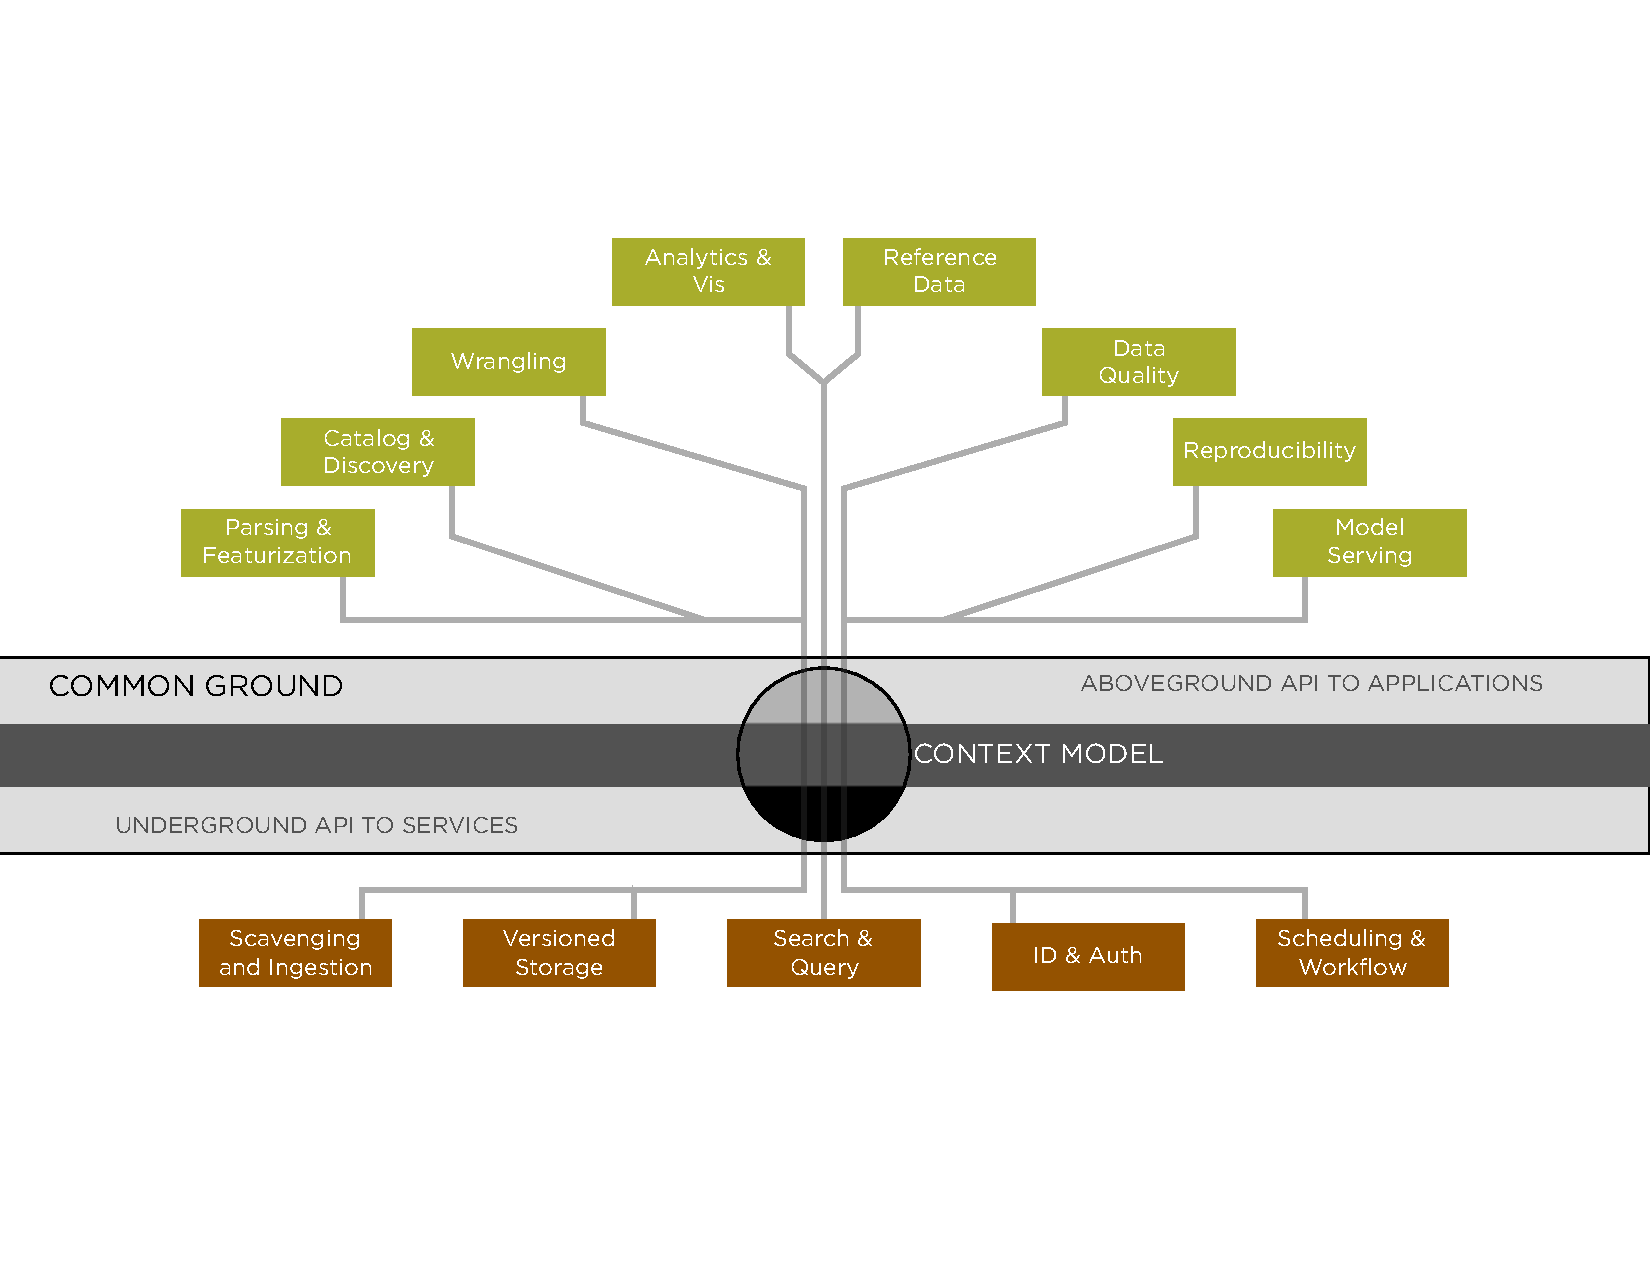
\includegraphics[width=0.75\linewidth]{groundarch.pdf}
  \caption{The initial architecture of Ground. \vikram{Can we replace this with the prettier version thats a little longer since we have space?}}
\label{fig:arch}
\end{figure*}
% \jmh{\textbf{Idea 3: A Pragmatic example in existing Hadoop workflows.  LinkedIn or Navigator customer story?}  Maybe take Idea 1 and make it less about assistive features, more about lost lineage across HDFS, Trifacta, Hive and Tableau?}

In a decoupled architecture of multiple applications and backend services, context serves as a ``narrow waist''---a single point of access for the basic information about data and its usage. It is hard to anticipate the breadth of applications that could emerge.
% However, the use of data context remains an open-ended design opportunity. 
Hence we were keen in designing Ground to focus on initial decisions that could enable new services and applications in future. 

\subsection{Design Requirements}
In our we were guided by Postel's Law of Robustness from Internet architecture: \emph{``Be conservative in what you do, be liberal in what you accept from others.''}  % <- Using American ." style instead of British ". style.
Guided by this philosophy, we identified four central design requirements for a successful data context service.

\smallitem{Model-Agnostic.} For a data context service to be broadly adopted, it cannot impose opinions on metadata modeling. 
Data models evolve and persist over time: modern organizations have to manage everything from COBOL data layouts to RDBMS dumps to XML, JSON, Apache logs and free text. 
As a result, the context service cannot 
prescribe 
%  dictate
how metadata is modeled---each dataset may have different metadata to manage. 
This is a challenge in legacy ``master data'' systems, and  a weakness in the Big Data stack today: Hive Metastore captures fixed features of relational schemas; HDFS captures fixed features of files.  
A key challenge in Ground is to design a core metamodel that captures generic information that applies to all data, as well as custom information for different data models, applications, and usage.
We explore this issue in Section~\ref{sec:metamodel}.

\smallitem{Immutable.} Data context must be immutable; \emph{updating} stored context is tantamount to erasing history. %Indeed, Postel's Law essentially dictates that we never discard information, lest somebody ask for it. 
There are multiple reasons why history is critical. 
The latest context may not always be the most relevant: we may want to replay scenarios from the past for what-if analysis or debugging, or we may want to study how context information (e.g., success rate of a statistical model) changes over time.
Prior context may also be important for governance and veracity purposes: we may be asked to audit historical behavior and metadata, or reproduce experimental results published in the past. 
This simplifies record-keeping, but of course it raises significant engineering challenges.  
We explore this issue in Section~\ref{sec:prototype}.

\smallitem{Scalable.} It is a frequent misconception that metadata is small. In fact, metadata scaling was already a challenge in previous-generation ETL technology. In many Big Data settings, it is reasonable to envision the data context being far larger than the data itself. Usage information is one culprit:  logs from a service can often outstrip the data managed by the service. Another is data lineage, which can grow to be extremely large
depending on the kind of lineage desired
~\cite{cheney2009provenance}.  Version history can also be substantial. 
We explore these issues in Section~\ref{sec:prototype} as well.

\smallitem{Politically Neutral.}  
Common narrow-waist service like data context must interoperate with a wide range of other services and systems designed and marketed by often competing vendors.
Customers will only adopt and support a central data context service if they feel no fear of lock-in; application writers will prioritize support for widely-used APIs to maximize the benefit of their efforts. 
It is important to note here that open source is not equivalent to political neutrality; customers and developers have to believe that the project leadership has strong incentives to behave in the common interest. 

\vspace{1em}
Based on the requirements above, the Ground architecture is informed by Postel's Law of Robustness and the design pattern of decoupled components. 
At its heart is a foundational metamodel called \emph{Common Ground} with an associated \emph{Aboveground} API for data management applications like the catalog and wrangling examples above. 
The core functions underneath Ground are provided by swappable component services that plug in via the \emph{Underground} API. 
A sketch of the architecture of Ground is provided in Figure~\ref{fig:arch}.


\subsection{Key Services}
Ground's functionality is backed by five decoupled subservices.  For agility, we are starting the project using existing open source solutions for each.  We anticipate that some of these will require additional features for our purposes. In this section we discuss the role of each subservice, and highlight some of the research opportunities we foresee.  Our initial choices for subservices are described in Section~\ref{sec:prototype}.

\smallitem{Ingest: Insertion, Crawlers and Queues}.  Metadata may be pushed into Ground or require crawling; it may arrive interactively or in batches. 
The main issue is to decouple the systems plumbing of ingest from an extensible set of metadata and feature extractors.
To this end, ingest has both Underground and Aboveground APIs.
New context metadata arrives for ingestion into Ground via an Underground queue API. 
As metadata arrives, Ground publishes notifications via an Aboveground queue. Aboveground applications can subscribe to these events to add unique value, fetching the associated metadata and data, and generating enhanced metadata asynchronously. 
For example, an application can subscribe for file crawl events, hand off the files to an entity extraction system like OpenCalais or DeepDive, and subsequently tag the corresponding Common Ground metadata objects with  the extracted entities.

Metadata feature extraction is an active research area; we hope that commodity APIs for scalable data crawling and ingest will drive more adoption and innovation in this area. 

\smallitem{Versioned Metadata Storage}.  Ground must be able to efficiently store and retrieve metadata with the full richness of the Common Ground metamodel, including flexible version management of code and data, general-purpose model graphs and lineage storage. 
% Ground also needs to reference external data and handle Schr\"{o}dinger versioning.  
While none of the existing open source DBMSs target this data model, one can implement it in a shim layer above many of them. 
We discuss this at greater length in Section~\ref{sec:perf}, where we examine a range of open-source DBMSs. As noted there, we believe this is an area for significant database research.

\smallitem{Search and Analyze}.  Access to context information in Ground is expected to be complex and varied. As is noted later, Common Ground supports arbitrary tags, which leads to a requirement for search-style indexing.
%; we plan to integrate Solr~\cite{solr} and ElasticSearch~\cite{elasticsearch}.  
Second, intelligent applications like those in Section~\ref{sec:scenarios} will run significant analytical workloads over metadata---especially usage metadata which could be quite large.  
Third, the underlying graphs in the Common Ground model require support for basic graph queries like transitive closures. 
Finally, it seems natural that some workloads will need to combine these three classes of queries.
%, perhaps via a federated query layer above them.  
As we explore in Section~\ref{sec:perf}, various open-source solutions can address these workloads at some level, but there is significant opportunity for research here.

\smallitem{Identity and Authorization}.  
Identity management and authorization are required for a context service, and must accommodate typical packages like LDAP and Kerberos.  
Note that authorization needs vary widely: the policies of a scientific consortium will differ from a defense agency or a marketing department.  
Ground's flexible metamodel can support a variety of relevant metadata (ownership, content labels, etc.) 
Meanwhile, the role of versioning raises
subtle security questions.
Suppose the authorization policies of a past time are considered unsafe today---should reproducibility and debugging be disallowed? 
More research is needed integrate
versions and lineage 
with security techniques like Information Flow Control~\cite{zeldovich2008securing} in the context of evolving real-world pipelines.

\smallitem{Scheduling, Workflow, Reproducibility}. 
We are committed to ensuring that Ground is flexible enough to capture the specification of workflows at many granularities of detail: from black-box containers to workflow graphs to source code.  
However, we do not expect Ground to be a universal provider of workflow execution or scheduling; instead we hope to integrate with a variety of schedulers and execution frameworks including on-premises and cloud-hosted approaches. 
This is currently under design, but the ability to work with multiple schedulers has become fairly common in the open source Big Data stack, so this may be a straightforward issue.

\smallitembot

\subsection{The Common Ground Metamodel}
\label{sec:metamodel}

\begin{figure}[th]
\centering
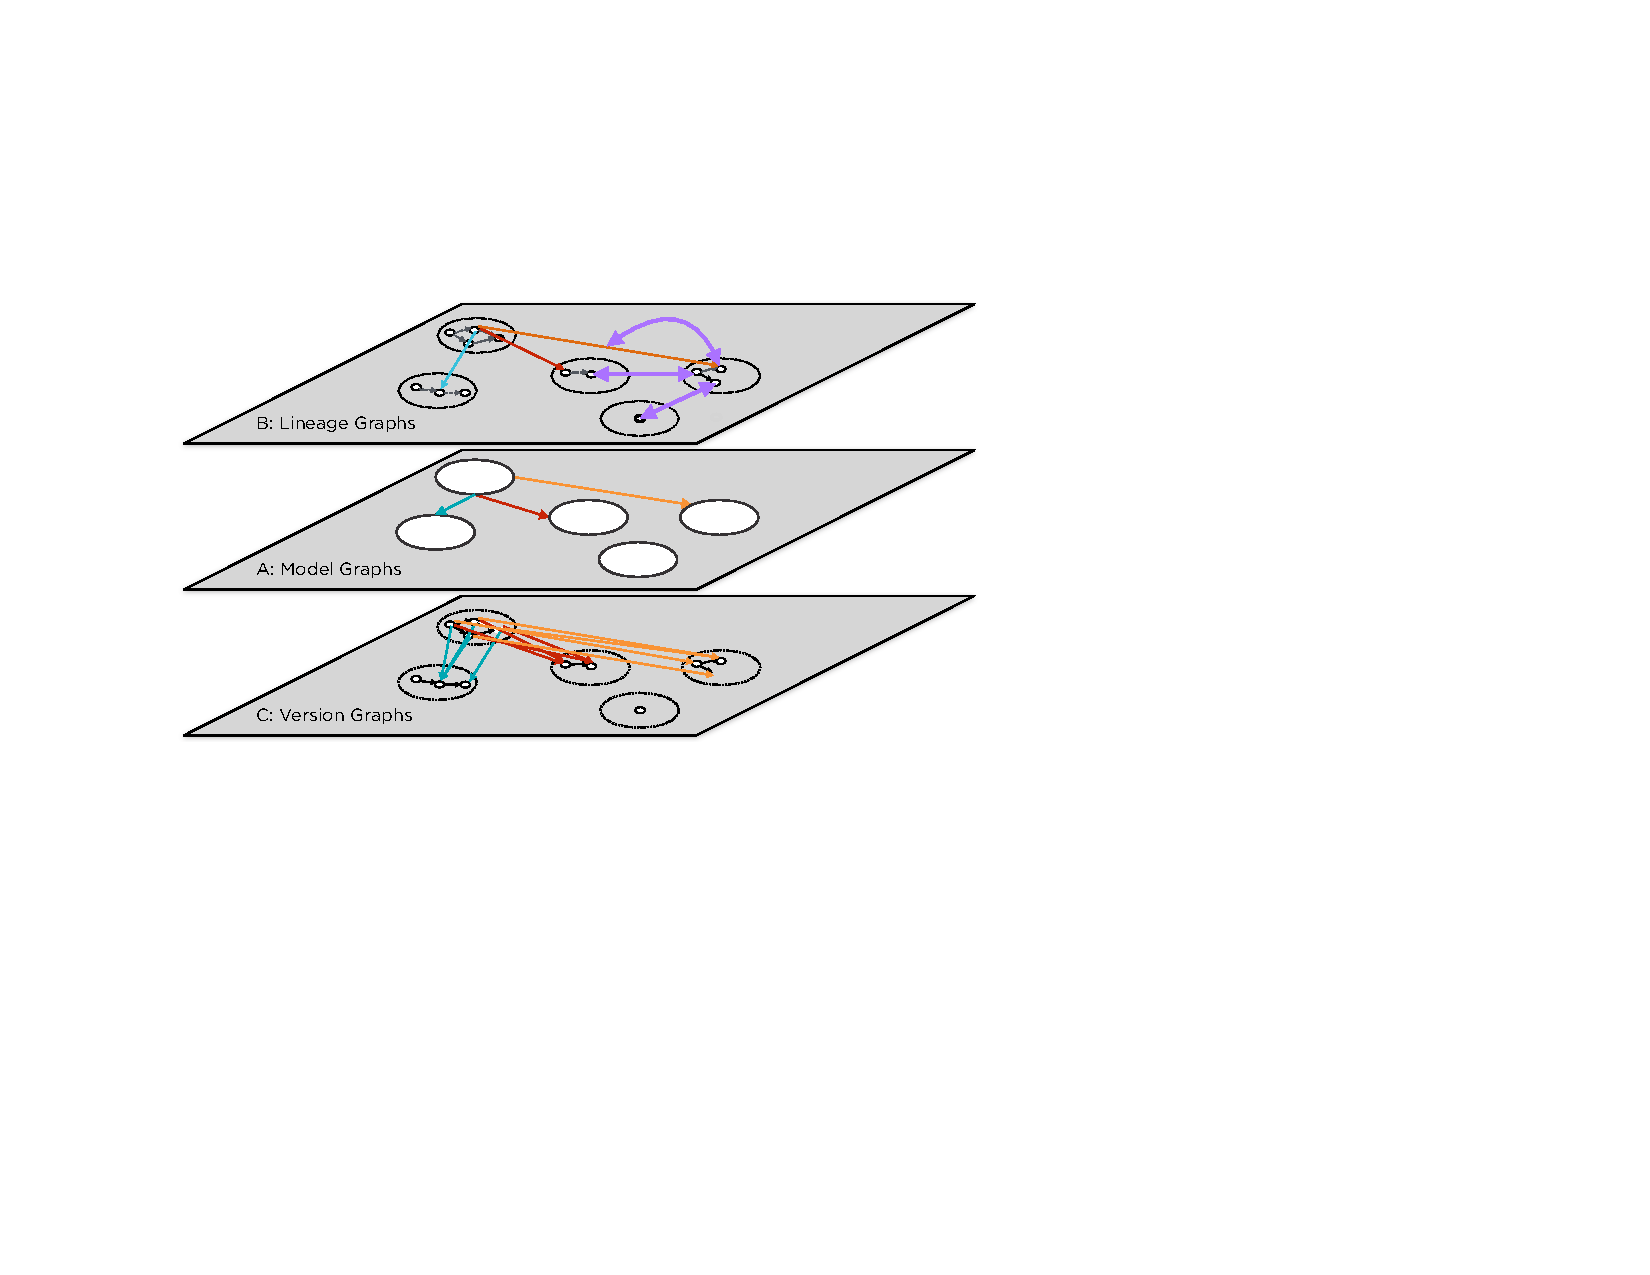
\includegraphics[width=\linewidth]{layers.pdf}
\caption{The Common Ground metamodel.} 
% The central layer shows {\node}s (circles) and {\edge}s.  
% Under are \kw{NodeVersion}s (small dots) corresponding to each \node, connected by \kw{EdgeVersion}s corresponding to each \edge.  
% Above is an example of lineage (dark edges) among selected versions.}
% For simplicity, the figure omits \kw{VersionSuccessor} relationships between different \kw{LineageEdgeVersion}s at the top, and between \
% \kw{EdgeVersion}s in the bottom layer.
\label{fig:layers}
\end{figure}

% \jmh{Pull in the practical motivation for each layer from the GDocs outline.}
Ground is designed to manage both the ABCs of data context and the design requirements of data context services.
The Common Ground metamodel is based on a layered graph structure shown in Figure~\ref{fig:layers}: one layer for each of the ABCs of data context.

\subsubsection{{\VersionGraph}s: Representing Change}

We begin with the \versiongraph layer of Common Ground, which captures changes corresponding to the \emph{C} in the ABCs of data context (Figure~\ref{fig:versioncode}).
This layer bootstraps the representation of all information in Ground, by providing the classes upon which all other layers are based. These classes and their subclasses are the only information in Common Ground that is not itself versioned; this is why it forms the base of the metamodel.

The main atom of our metamodel is the \version, which is simply a globally unique identifier; it represents an immutable version of some object; we
depict \version{}s via the small circles in the bottom layer of Figure~\ref{fig:layers}. \vikram{two semicolons in this sentence.}
Ground links {\version}s into \kw{VersionHistoryDAG}s via \kw{VersionSuccessor} edges
indicating that one version is the descendant of another (the short dark edges in the bottom of Figure~\ref{fig:layers}.)
Type parametrization ensures that all of the \kw{VersionSuccessor}s in a given DAG link the same subclass of {\version}s together.
This representation of DAGs captures any partial order, and is general enough to reflect multiple different versioning systems.

\kw{RichVersion}s support customization. These variants of \version{}s can be associated with
ad hoc {\gtag}s (key-value pairs) upon creation. Note that all of the classes introduced above are immutable---new values require the creation of new \version{}s.

\subsubsection{{\ModelGraph}s: Application Context}
% Our philosophy is that the metamodel should be designed in layers for
% simplicity and elegance. \versiongraph classes are shared and evolve in infrequent,
% regimented updates to maximize backwards compatibility. More detailed versions
% of the metamodel (including versions specific to use cases) are mapped onto
% simpler versions of the model. Our goal to find a balance between the
% simplicity and the expressivity of the metamodel and leave the rest up to the
% application using this metamodel.

% To illustrate this philosophy, we have developed a somewhat richer metamodel
% that can be imposed onto the aforementioned model.

The \modelgraph level of Common Ground provides a model-agnostic representation of application metadata: the \emph{A} of our ABCs (Figure~\ref{fig:modelcode}.) 
We use a graph model for flexibility: graphs can represent metadata entities and relationships from
semistructured (JSON, XML) and structured (Relational, Object-Oriented, Matrix) data models. A simple graph model enables 
the agility of schema-on-use at the metadata level, allowing diverse metadata to be independently captured as ad hoc model graphs and 
integrated as needed over time.

The \modelgraph is based on an internal superclass called \itemground, which is simply a unique ID that can be
associated with a \kw{VersionHistoryDAG}. Note that 
an \itemground is intrinsically immutable, but can capture change via its associated \kw{VersionHistoryDAG}: a fresh
\version of the \itemground is created whenever a \gtag is changed. 

Ground's public API centers around three core object classes derived from \itemground: {\node}, {\edge}, and {\graph}.
Each of these subclasses has an associated subclass in the \versiongraph: \kw{NodeVersion}, \kw{EdgeVersion} and \kw{GraphVersion}. {\node}s and 
{\edge}s are highlighted in the middle layer of Figure~\ref{fig:layers}, with the {\node}s projected visually onto 
their associated versions in the other layers.


\begin{figure}[H]
\begin{scriptsize}
% \begin{multicols}{2}
\lstinputlisting{version.java}
% \end{multicols}
\end{scriptsize}
% \vspace{2em}
  \caption{Java skeleton for Version classes in Common Ground. Methods have been elided. Full code is available at \texttt{https://github.com/ground-context/ground}. \vikram{Can we get rid of the Jackson annotations? They're not particularly informative, I don't think.}}
\label{fig:versioncode}
\end{figure}

The \versiongraph allows for ad hoc {\gtag}s, but many applications desire more structure.
To that end, the \modelgraph includes a subclass of \itemground called {\structure}. A \structure is like a schema: a set of {\gtag}s that must be present. Unlike database schemas, the \structure class of Ground is versioned, via a \kw{StructureVersion} subclass in the \versiongraph.  If an \itemground is associated with a \structure, each \version of the \itemground is associated with a corresponding \kw{StructureVersion} and must define those {\gtag}s (along, optionally, with other ad hoc {\gtag}s.)
Together, {\gtag}s, {\structure}s and \kw{StructureVersion}s enable a breadth of metadata representations: from unstructured to semi-structured to structured.

\smallitem{External Items and Schr\"{o}dinger Versioning}\\
\jmh{We don't have External Items explicit in the pseudocode. Should we? If not we need to reword this 
section to be less ``object-oriented'' and more conceptual.}
\vikram{Adding it wouldn't be too hard. Do you think it's worth it? We had these at one point, I think in the Scala version, but sort of ended up folding them into regular versions.}
We often wish to track items whose metadata is managed outside of Ground: canonical examples
include GitHub repositories and Google Docs. Ground cannot automatically track these items as they change.
They are represented in Ground by \kw{ExternalItem}s, with \kw {ExternalVersion}s that contain various tags: a \kw{timestamp}, optional \kw{cachedValue}, and parameters for accessing the
reference (e.g., port, protocol, URI, etc.) 
Whenever a Ground client uses the Aboveground API to access an a \kw{ExternalVersion}, this results in Ground fetching the object and generating a new \kw{ExternalVersion}, containing a new
\kw{VersionID}, an updated timestamp and possibly an updated cached value. We refer to this as a \emph{Schr\"{o}dinger} versioning scheme: each time we observe an \kw{ExternalItem} it changes. This allows Ground to track the history of an external object \emph{as perceived} by Ground-enabled applications.

\begin{figure}[bh]
\begin{scriptsize}
\lstinputlisting{model.java}
\end{scriptsize}
\caption{Java skeleton for Model classes.}
\label{fig:modelcode}
\end{figure}


\smallitem{SuperVersions: An Implementation Detail.}
\begin{figure}[th]
\centering
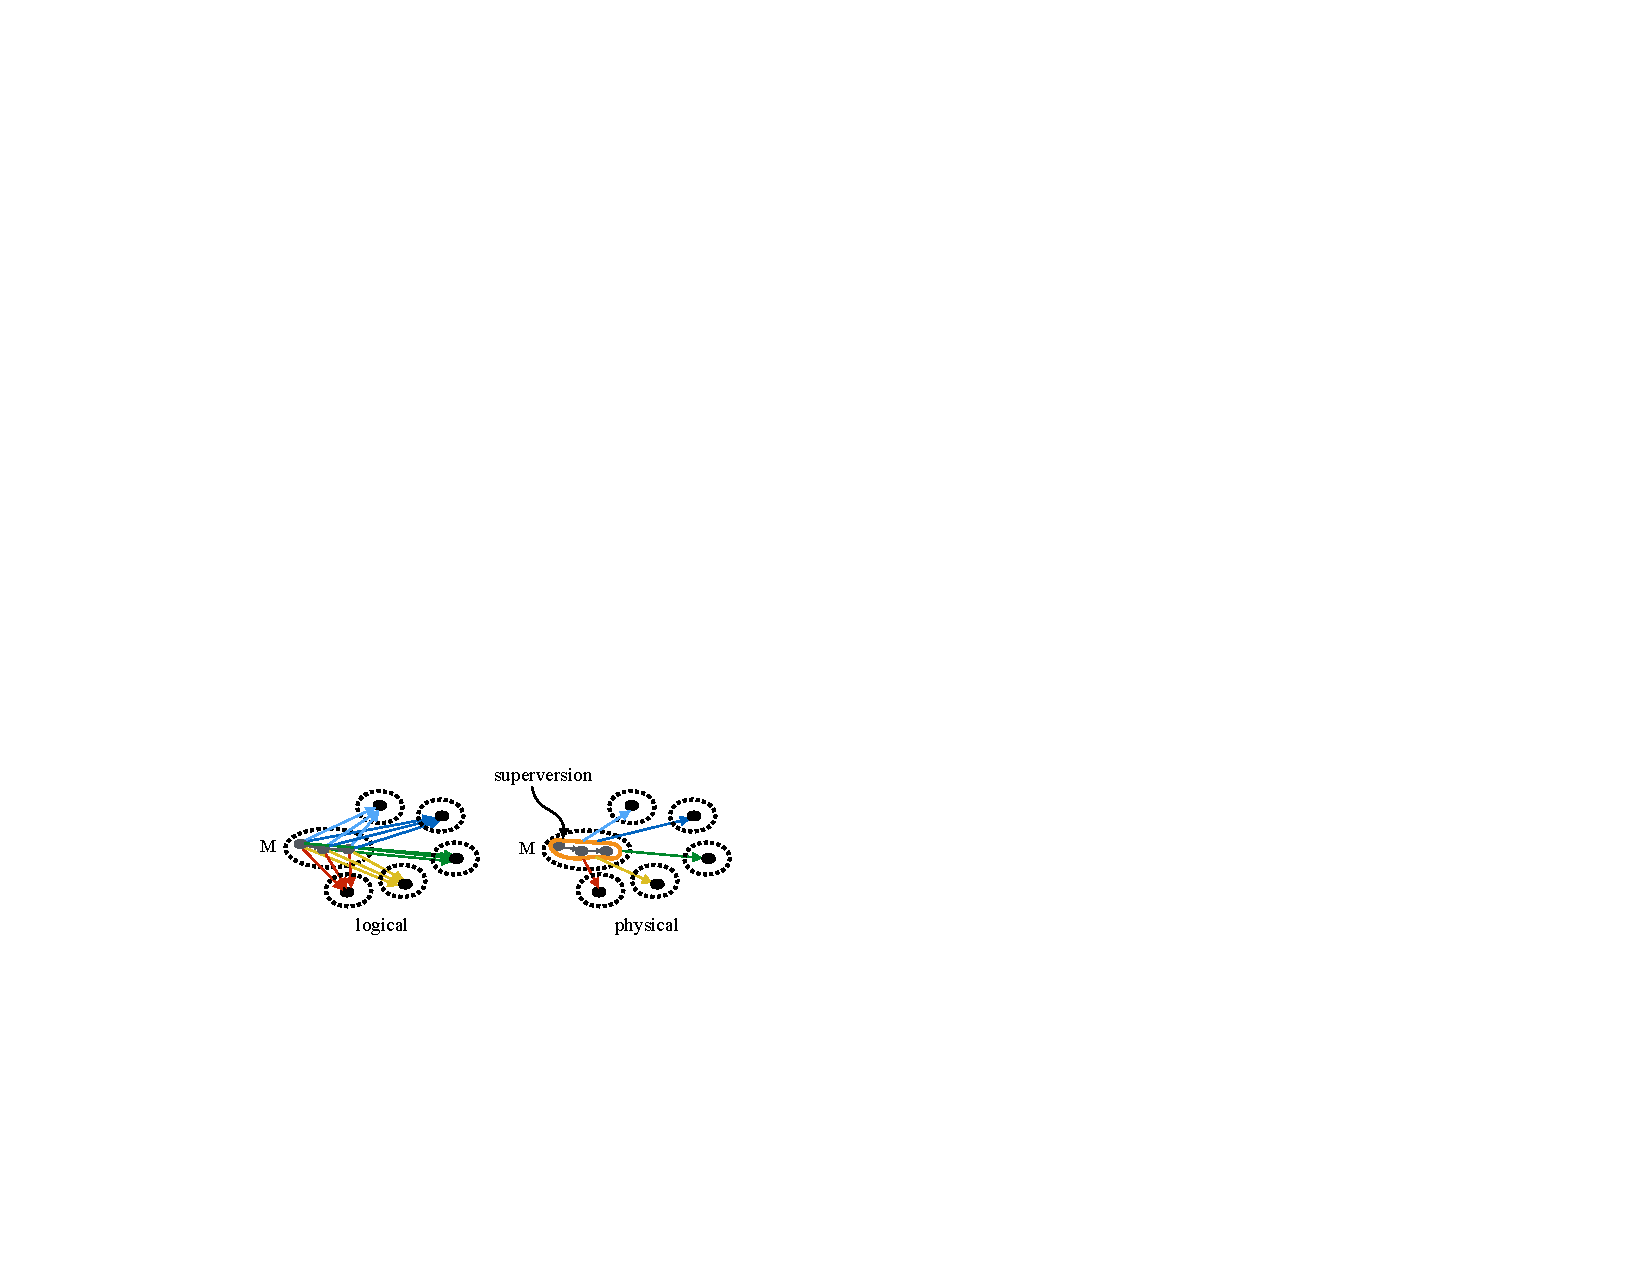
\includegraphics[width=\linewidth]{superversion.pdf}
\caption{VersionGraph with 2 changes to a single node, in logical and physical (SuperVersion) representations.}
\label{fig:superversion}
\end{figure}
The Common Ground model captures versions of relationships (e.g., \edge{}s) between versioned objects (e.g., \node{}s). The relationships themselves are first-class objects with identity and tags. Implemented naively, the version history of relationships can grow in unintended and undesirable ways. We address that problem by underlaying the logical Common Ground model with a physical compression scheme combined with lazy materialization of logical versions.

Consider updating the current version 
%$m_v$ 
of a central \node{} $M$
with $n$ incident \edge{}s to neighbor \node{}s.
Creating a new \kw{NodeVersion} for $M$ implicitly requires creating $n$ new \kw{EdgeVersion}s, one for each of the $n$ incident edges, to capture the connection between the new version of $M$ and the (unchanged!) versions of the adjacent nodes. More generally, the number of \kw{EdgeVersion}s grows as the product of node versioning and node fanout. 
% $m_v$ is connected to versions of its $n$ neighboring \node{}s via \kw{EdgeVersion}s $e^1_v1 \ldots e^n_vn$.
 % If we create a new version $m_{v+1}$ of $M$, we implicitly need new \kw{EdgeVersions} for all the $n$ incident \edge{}s, to represent the fact that $m_{v+1}$ is connected to the (unchanged!) versions of the $n$ neighbor nodes. 

We can mitigate the version factor by using a \kw{SuperVersion}, an implementation detail that does not change the logical metamodel of Common Ground. In essence, \kw{SuperVersion}s capture a compressed set of contiguous \kw{NodeVersion}s and their common adjacencies. If we introduce $k-1$ changes to version $v$ of node $M$ before we change any adjacent node, there will be $k$ logical \kw{EdgeVersion}s connecting $M$ to each of its neighbor \kw{NodeVersion}s. Rather than materializing those \kw{EdgeVersion}s, we can use a \kw{SuperVersion} capturing the relationship between each neighbor and the range $[v, vk]$ (Figure~\ref{fig:superversion}). The actual logical \kw{EdgeVersion}s can be materialized on demand by the Ground runtime. More generally, in a branching version history, a \kw{SuperVersion} captures a growing rooted subgraph of the \version{}s of one \itemground, along with all adjacent \version{}s. A \kw{SuperVersion} grows monotonically to encompass new \version{}s with identical adjacencies. Note that the \kw{SuperVersion} represents both a supernode \emph{and the adjacent edges to common nodes}; directionality of the adjacent edges is immaterial.   
% We can use \kw{SuperVersion}s for any relationship between versioned \itemground{}s: the \edge{}s between \node{}s, the relationship of \kw{StructureVersion}s to \kw{RichVersion}s, etc. \jmh{This discussion is a bit broken because \itemground is a subclass of \version rather than the other way round.  Why is that?}


\subsubsection{{\LineageGraph}s: Behavior}
\begin{figure}[bh]
\begin{scriptsize}
\lstinputlisting{lineage.java}
\end{scriptsize}
\caption{Java skeleton for Lineage classes.}
\label{fig:lineagecode}
\end{figure}

The goal of the \lineagegraph layer is to capture usage information composed from the nodes and edges in the model graph (Figure~\ref{fig:lineagecode}.)  
To facilitate data lineage, Common Ground depends on two specific items---
principals and workflows---that we describe here.
% These are the only two items in Common Ground that go beyond graph structure; they are fundamental to the semantic notion of lineage.

\kw{Principal}s (a subclass of \node) represent the actors that work with data:  users, groups, roles, etc. 
\kw{Workflow}s (a subclass of {\graph}) represent specifications of code that can be invoked. Both of these classes have associated \kw{Version} subclasses.
Any Data Governance effort requires these classes: as examples, they are key to
authorization, auditing and reproducibility.

In Ground, lineage
is captured as a relationship between two {\version}s. 
This relationship is due to some process, either computational
(a workflow) or manual (via some principal). \kw{LineageEdgeVersion}s (purple arrows in the top layer of Figure~\ref{fig:layers}) connect two or more (possibly differently-typed) {\version}s, at least one of which is a \kw{Workflow} or \kw{Principal} node. 
Note that \kw{LineageEdgeVersion} is not a subclass of \kw{EdgeVersion}; an \kw{EdgeVersion} can only connect two \kw{NodeVersion}s; a \kw{LineageEdge} can connect {\version}s from two different subclasses, including subclasses that are not under \kw{NodeVersion}.  
For example, we might want to record that Sue imported \kw{nltk.py} in her \kw{churn.py} script; this is captured by a \kw{LineageEdge} between a \kw{PrincipalVersion} (representing Sue) and an \kw{EdgeVersion} (representing the dependency between the two files).  

% \jmh{This paragraph can be chopped for space.}
% Usage data is often generated by analyzing log files, code, and/or data, and it can become very large.
% There are important choices about how and when to materialize lineage that are best left to applications. For example, in a pure SQL environment, the lineage of a specific tuple in a table might be materialized on demand as a tree of input tuples, but the lineage for all tuples in the table is more efficiently described by version IDs for the SQL query and its input tables. Ground can support both, but 
% does not dictate a choice.
% % To support such lazy evaluation, \emph{ephemeral} \kw{LineageEdgeVersion}s can be generated in the Ground lineage API without materializing the (redundantly computed) \kw{LineageEdgeVersion}s in immutable storage. 
% % \vikram{I'm confused about what this is saying. 
% % It definitely doesn't exist in the code. :-)}

\subsubsection{Extension Libraries}
The three layers of the Ground metamodel are deliberately general-purpose and non-prescriptive.
We expect Aboveground clients to define custom \kw{Structure}s to capture reusable application semantics.  
These can be packaged under {\node}s representing shared libraries---e.g., a library for representing
relational database catalogs, or scientific collaborations. \kw{StructureVersion}s allow these to be evolved over time in an identifiable manner.

% The API for \groundwire is the subject of a separate document.

%%%%%%%%%%%

\subsection{\texttt{Grit}: An illustrative example}
\begin{figure*}[th]
\centering
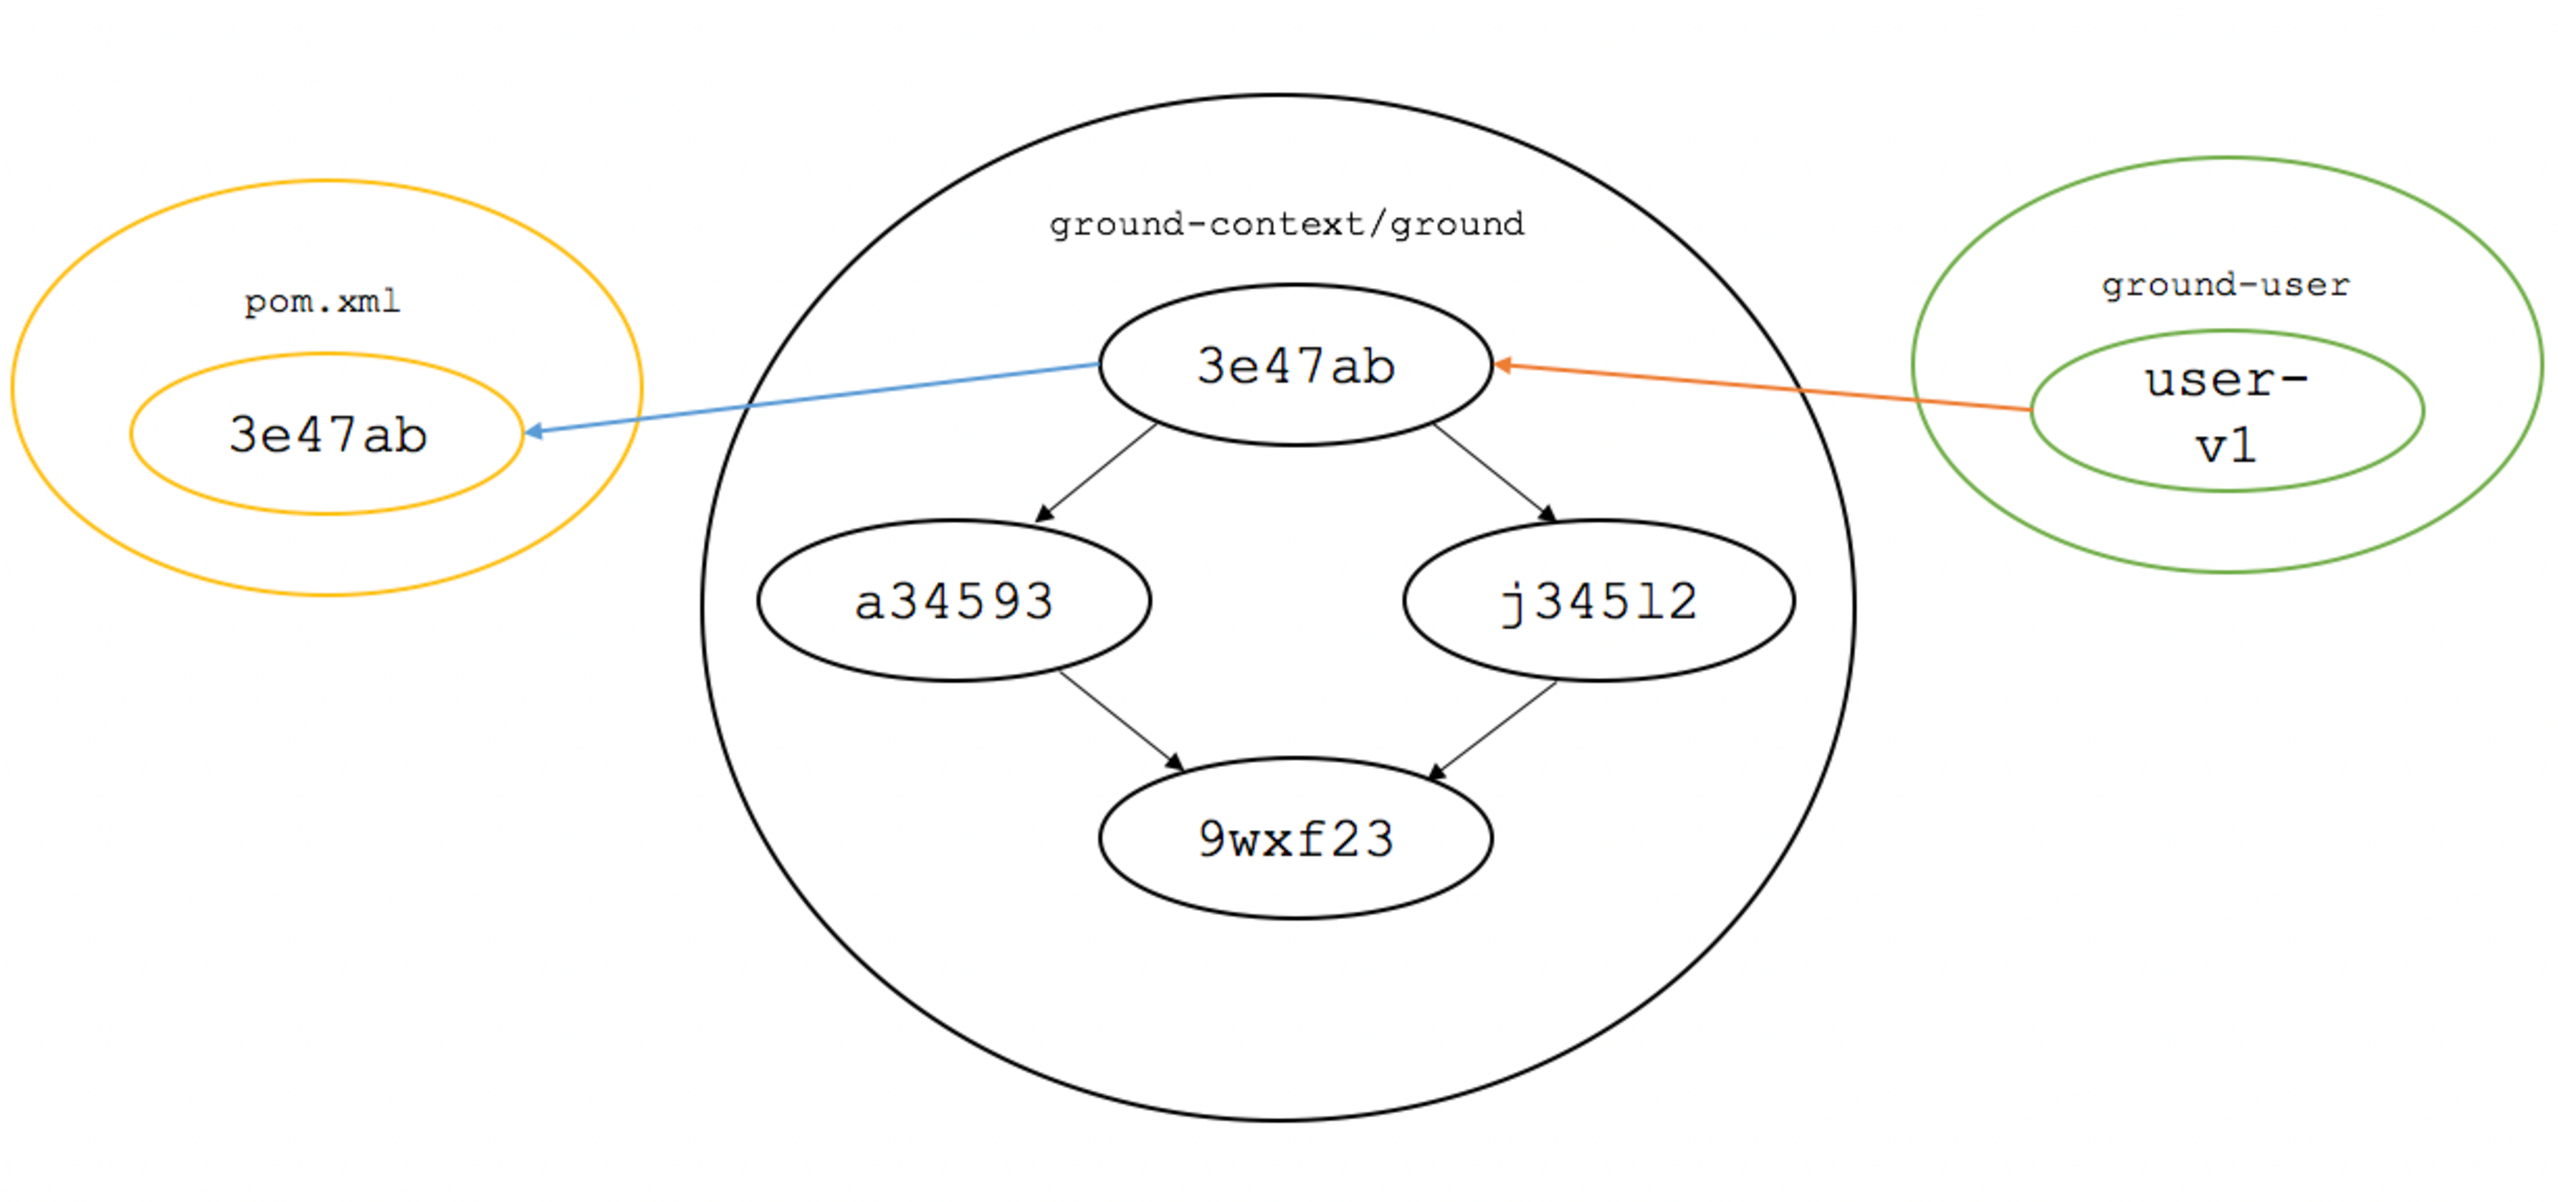
\includegraphics[width=0.75\linewidth]{grit.pdf}
\caption{An illustration of the data structure involved in the grit example.}
\label{fig:grit}
\end{figure*}

% \jmh{Would be good to have the data structures in a Figure, and simple pseudocode example to be able to refer to here where we create a node, create node versions, show version successors, Edge, edgeversions, etc.}
To demonstrate the flexibility and expected usage of our model, we discuss an aboveground service we built called Grit: the Ground-git tracker. Grit maps metadata from git repositories into Ground, allowing users to easily associate contextual information about code (e.g., transformation or analysis scripts) with metadata about data (the inputs and outputs of the script).

% \jmh{Maybe we want to illustrate the use of Structures via commitHash on the Repo node, and the use of Tags via a Ground user annotation?}
Consider a git repository on Github, such as \texttt{ground-context/ground}. This repository's identity is represented by a \node in Ground (the black circle in Figure~\ref{fig:grit}), which we will call $R$ for the sake of discussion. Every time a developer commits changes to the repository, git generates a unique hash that corresponds to a new version of the repository. Each one of these versions will be associated with a \structure that specifies two tags, a \kw{commitHash} and a \kw{commitMessage} (not pictured). Every version of the repository must have tags with both those keys specified.  grit registers a hook with Github to be notified about these commits and their hashes. Upon being notified of a new commit hash, grit calls a Ground API to register this new version of $R$; Ground stores this as a \kw{NodeVersion} associated with $R$, containing a \kw{commitHash} tag. The API also allows grit to specify the commit hashes that preceded this new version; Ground internally relates each \kw{NodeVersion} to its predecessor(s) via \kw{VersionSuccessor}s\footnote{Note that aboveground applications do not explicitly create \kw{VersionSuccessor}s; the Ground API for registering a new \kw{NodeVersion} and its parent(s) captures information that Ground uses to generate the \kw{VersionSuccessor}s internally.} (the black arrows in Figure~\ref{fig:grit}). 

To extend the example, grit can be augmented to track files (the yellow circle in Figure~\ref{fig:grit}) as well as repositories. Grit represents each file in Ground via a \node, with an \edge (the blue arrow in Figure~\ref{fig:grit}) between each file and the repository \node. Upon hearing of a commit from Github, grit interrogates git to determine which files changed in that commit. For a given file $F$ that has changed, Grit creates a new \kw{NodeVersion} with metadata about the file (e.g. a size and checksum). Moreover, a new \kw{EdgeVersion} associates the new file version with the new repository version.

Lastly, we can model users (the green circle in Figure~\ref{fig:grit}) and the actions they perform. Once more, each user will be represented by a \node, which will be updated whenever the attributes of the user change -- normally, not very often. There would be a \kw{LineageEdge} (the orange arrow in Figure~\ref{fig:grit}) that represents the changes that a user has caused in the repository. Each \kw{LineageEdgeVersion} in this \kw{LineageEdge} points from the user \kw{NodeVersion} to the repository commit \kw{NodeVersion}, implying that the changes the user made are represented in this commit.

The initial grit example was chosen to be simple but useful; of course it would need substantial extensions to capture every aspect of git's metadata, but it's unclear that users desire that level of detail to be captured for integration with other context. Moving beyond git, we believe that the generality of the Common Ground metamodel will allow users to capture a wide variety of use cases. We have currently developed basic extension libraries that allow Ground to capture relational metadata and file system metadata, in addition to git; we hope that more contributions will be forthcoming given the simplicity and utility of the Common Ground model.

\section{Ground 0}
\label{sec:prototype}

% \subsection{State of the System}
Our initial Version 0 of Ground implements the Common Ground metamodel and provides REST APIs for interaction with the system. 
Referring back to Figure~\ref{fig:arch}, Ground 0 uses Apache Kafka for the Aboveground API (to enable Aboveground applications to subscribe to events), and to enable queuing of bulk underground APIs such as the Crawling/Ingest API.
Ground 0 makes use of LinkedIn's Gobblin system for crawling and ingest from files, databases, web sources and the like.
We have integrated and evaluated a number of backing stores for versioned storage, including PostgreSQL, Cassandra, TitanDB and Neo4j; we report on results later in this section.
We are currently integrating ElasticSearch for text indexing and are still evaluating options for ID/Authorization and Workflow/Scheduling. 

To exercise our initial design and provide immediate functionality,
we built support for three sources of metadata most commonly used in the Big Data ecosystem: file metadata from HDFS, schemas from Hive, and code versioning from git.
To support HDFS, we extended Gobblin to extract file system metadata from its HDFS crawls and publish to Ground's Kafka connector. The resulting metadata is then ingested into Ground, and notifications are published on a Kafka channel for applications to respond to. To support Hive, we built an API shim that allows Ground to serve as a drop-in replacement for the Hive Metastore.
One key benefit of using Ground as Hive's relational catalog is Ground's built-in support for versioning, which---combined with the append-only nature of HDFS---makes it possible to \emph{time travel} and view Hive tables as they appeared in the past.  To support git, we have built crawlers to extract git history graphs as \kw{ExternalVersion}s in Ground. These three scenarios guided our design for Common Ground.

Having initial validation of our metamodel on a breadth of scenarios, our next concern has been the efficiency of storing and querying information represented in the Common Ground metamodel, given both its general-purpose \modelgraph layer, and its support for versioning. To get an initial feeling for these issues, we began with two canonical use cases:

\smallitem{Proactive Impact Analysis.} A common concern in managing operational data pipelines is to assess the effects of a code or schema change on downstream services.
As a real-world model for this use case, we took the source code of Apache Hadoop and constructed a dependency graph of file imports that we register in Ground.
We perform impact analysis by running transitive closure starting from 5,000 randomly chosen files, and measuring the average time to retrieve the transitively dependent file versions.

\smallitem{Dwell Time Analysis.} In the vein of the analysis pipeline Sue manages in Section~\ref{sec:scenarios}, our second use case involves an assessment of code versions on customer behavior. 
In this case, we study how user ``dwell time'' on a web page correlates with the version of the software that populates the page (e.g., personalized news stories). 
We used a sizable real-world web log ({\small \url{http://waxy.org/2008/05/star_wars_kid_the_data_dump/}}) %~\cite{starwarskid}, 
but had to simulate code versions for a content-selection pipeline. 
To that end we wanted to use real version history from git; in the absence of content-selection code we used the Apache httpd web server repository. 
Our experiment breaks the web log into sessions and artificially maps each session to a version of the software.
We run 5,000 random queries choosing a software version and looking up all of its associated sessions.
\smallitembot

While these use cases are less than realistic both in scale and in actual functionality, we felt they would provide simple feasibility results for more complex use cases.

\subsection{Initial Experiences}
\label{sec:perf}
To evaluate the state of off-the-shelf open source, we chose leading examples of relational, NoSQL, and graph databases.
All benchmarks were run on a single Amazon EC2 \kw{m4.xlarge} machine with 4 CPUs and 16GB of RAM. 
Our initial goal here was more experiential than quantitative---we wanted to see if we could easily get these systems to perform adequately for our use cases and if not, to call more attention to the needs of a system like Ground.
We acknowledge that with further tuning, these systems might perform better than they did in our experiments, though we feel these experiments are rather fundamental and should not require intensive tuning.

\begin{figure}
\centering
\begin{minipage}{.5\linewidth}
  \centering
  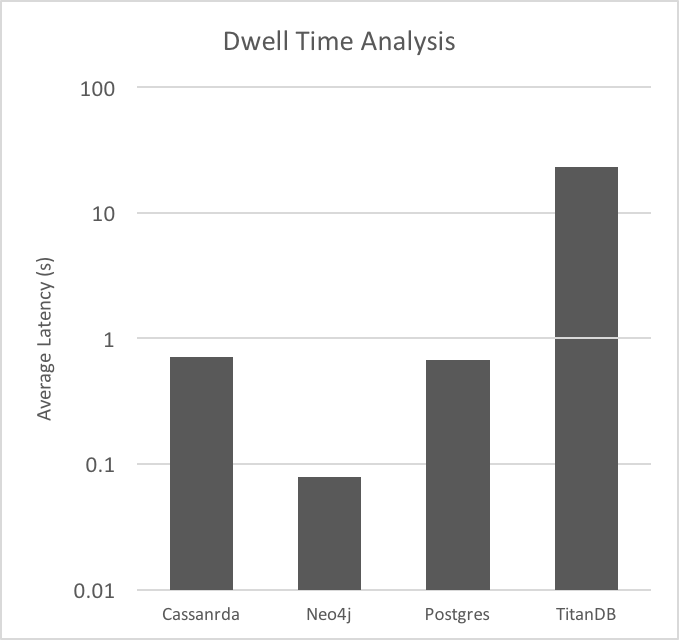
\includegraphics[width=\linewidth]{adjacent.png}
  \caption{Dwell time analysis.}
  \label{fig:dwell}
\end{minipage}%
\begin{minipage}{.5\linewidth}
  \centering
  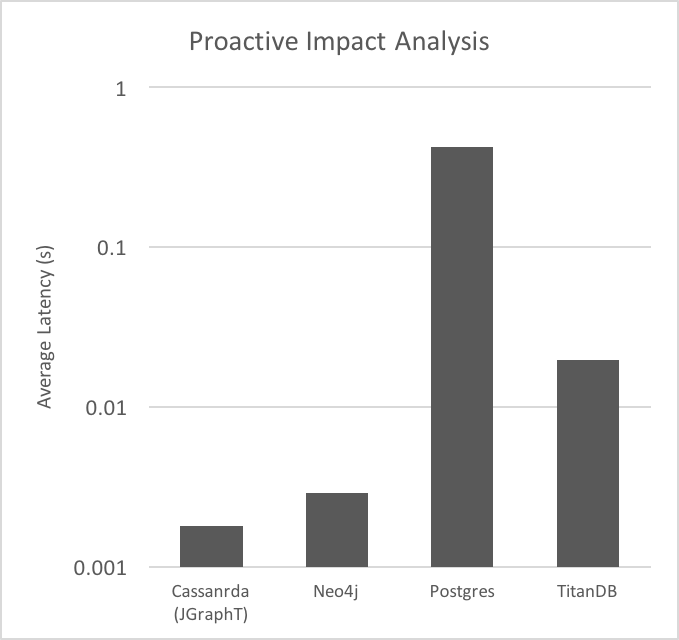
\includegraphics[width=\linewidth]{trans_closure.png}
  \caption{Impact analysis.}
  \label{fig:impact}
  \end{minipage}
 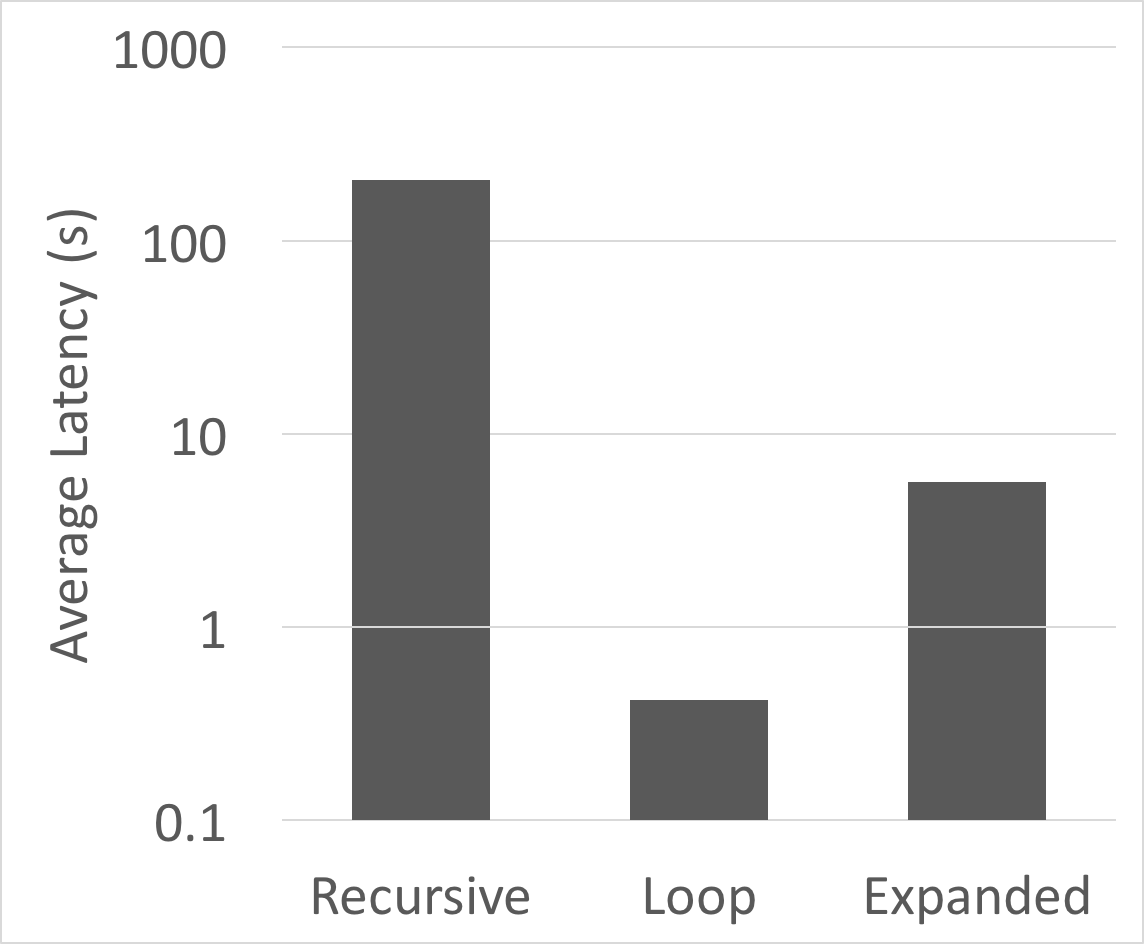
\includegraphics[width=0.5\linewidth]{postgres.png}
  \caption{PostgreSQL transitive closure variants.}
  \label{fig:postgres}
\end{figure}


\smallitem{PostgreSQL}. We normalize the Common Ground entities 
(\itemground, \version, etc.) into tables, and the relationships
(e.g., \kw{EdgeVersion}) into tables with indexes on both sides. 
The dwell time analysis amounts to retrieving all the sessions corresponding to a server version; it is simply a single-table look-up through an index. The result set was on the order of 100s of nodes per look-up.

For the impact analysis experiment, we compared three PostgreSQL implementations. The first was a \kw{WITH RECURSIVE} query. 
The second was a UDF written in PGPLSQL that computed the paths in a (semi-naïve) loop of increasing length. 
The last was a fully-expanded 6-way self-join that computed the paths of the longest possible length. Figure~\ref{fig:postgres} compares the three results; surprisingly, the UDF loop was faster than the native SQL solutions. 
Figure~\ref{fig:impact} shows that we were unable to get PostgreSQL to be within an order of magnitude of the graph processing systems. 

\smallitem{Cassandra}. In Cassandra, every entity and relationship from the Common Ground model is represented as a key/value pair, indexed by key. 
The Cassandra dwell time analysis query was identical to the Postgres query: a single table look-up which was aided by an index.
Cassandra doesn't support recursive queries; for impact analysis, we wrapped Cassandra with JGraphT, an in-memory Java graph-processing library. We did not count the time taken to load the graph into JGraphT from Cassandra, hence Figure~\ref{fig:impact} shows a very optimistic view of Cassandra's performance for this query.

\smallitem{Neo4j}. Neo4j is a (single-server) graph database, so modeling the Common Ground graphs was straightforward.
The average Neo4j dwell time analysis was fast; the first few queries were markedly slow
(${\sim}10$ seconds),
but subsequent queries were far faster, presumably due to caching. 
Neo4j excelled on transitive closure, performing only 50\% slower than in-memory JGraphT.

\smallitem{TitanDB}. TitanDB is a scale-out graph database designed to run over a NoSQL database like Cassandra, which is how we deployed it in our experiments on a single machine. % \jmh{right?} 
Once again, mapping our graph-based model into TitanDB was straightforward.
TitanDB's dwell time analysis performance was significantly slower than the rest of the systems, despite indexing.
The impact analysis query was significantly faster than any Postgres implementation but was still an order of magnitude slower than Neo4j and JGraphT. 

\smallitembot
While there is variance in our simple dwell time analysis lookups, the bigger divergence is in the impact analysis workload.
We can expect impact analysis to traverse a small subgraph within a massive job history. Queries on small subgraphs should be very fast---ideally as fast as an in-memory graph system~\cite{mcsherry2015scalability}. JGraphT-over-Cassandra and Neo4j provide a baseline, though neither solution scales beyond one server. PostgreSQL and TitanDB do not appear to be viable even for these modest queries. Of these systems, only Cassandra and TitanDB are designed to scale beyond a single server.

% \section{Discussion}
% \label{sec:discussion}
% \jmh{This may evolve into Research Opportunities or Future Work, but this is a placeholder for things that were postponed in earlier text}

% \jmh{Backref to Scalability discussion above, and the question ``are logs data or metadata''?}
% Functionality: well, we've started building out a few things and they went well.  Apiary and Grit.

% Performance: Here we ran into some bottlenecks with the widely-used storage systems in the field.  This merits more attention.

% \section{Challenges for the community}
% \label{sec:challenges}
% \jmh{May not be room for this. Instead find a way to call out the challenges in the body as they occur, with clear formatting.}

\section{Related Work}
\label{sec:relwork}
% \joey{made a pass on this section and it looks good}
Work related to this paper comes in a variety of categories. 
\jmh{Address this?  For submission brevity, we focus on related system architectures and omit bibliography entries to systems easily found online. 
An accepted version will contain a more scholarly bibliography.}


% Legacy 
Classic commercial Master Data Management and ETL solutions were not designed for 
schema-on-use or agility. 
Still, they influenced our thinking and many of their features should be supportable as a subset of the Ground functionality~\cite{loshin2010master}.

Meanwhile,
two emerging metadata systems address governance for Big Data: Cloudera Navigator and the Hortonworks-led Apache Atlas. 
Both provide graph models that inspired the Common Ground \modelgraph; neither provides versioning or is perceived as vendor-neutral. % These systems are also exploring ``underground'' alternatives for storage.

There is a broad space of efforts that illustrate the possibilities of data context. 
There are many commercial applications and research projects for Aboveground tasks: cataloging, wrangling, lineage analysis, query and workflow management, information extraction, ontology management, etc. 
OpenChorus and IBM LabBook provide overarching portals for collaboration on data projects.
LinkedIn WhereHows, FINRA Herd and Google Goods are metadata services built to support the evolving data workflows in their respective organizations. Goods is a particularly mature system, bundling what we call Underground services with various proprietary services we might describe as Aboveground applications.
All of the above make use of specific metamodels customized to their needs. By contrast, Ground is focused on designing a reusable service to enable diverse applications and organizations to integrate their notions 
of data context. 
This shapes the core challenges and opportunities we are pursuing, and hopefully will encourage adoption and innovation.

\section{Future Work}
In the spirit of agility, we view Ground as a work in progress. Our intent is to keep Common Ground simple and stabilize it relatively quickly, with evolution and innovation happening largely outside the system core. In the main, our goal is to facilitate continued innovation from the community: in systems belowground, and algorithms and interfaces aboveground.

\subsection{Ground}
Within Ground proper, we want to make it increasingly easy to use, by offering developers higher levels of abstraction for the existing Common Ground API.  One direction we envision is a library of common ``design patterns'' for typical data models. Many of the use cases we have encountered revolve around relational database metadata, so a design pattern for easily registering relational schemas is an obvious first step, and one that can build on our experience with our Hive metastore implementation. A related direction we hope to pursue is a more declarative interface for specifying models, involving simple relationships and constraints between collections or object classes. This would be a good fit for capturing metadata from typical database-backed applications, like those that use Object-Relational Mappings. From such high-level specifications, Ground could offer default (but customizable) logic for managing versioning and lineage.

\subsection{Underground}
Underground, as we emphasize above, we see open questions regarding the suitability of current database systems for the needs of data context. Our initial assessment suggests a need for more work: both a deeper evaluation of what exists and very likely designs for something new. 

As of now, part of the challenge is to understand relevant workloads for Ground deployments.  Our examples to date are limited, but given the diversity of participants in the early stage of the project we foresee a quick learning curve. Three simple patterns have emerged from early discussion: tag (attribute) search, wrangling/analysis of usage logs, and traversal (especially transitive closure) of graphs for lineage, modeling and version history. The right solution for this initial workload today is unclear on a number of fronts. First, existing systems for the three component workloads are quite different from each other; there is no obvious single solution. Second, there are no clear scalable open source ``winners'' in either log or graph processing. Leading log processing solutions like Splunk and SumoLogic are closed-source and the area is not well-studied in research. There are many research papers and active workshops on graph databases (e.g., \cite{grades16}), but we found the leading systems lacking.  Third, we are sensitive to the point that some problems---especially in graphs---prove to be smaller than expected, and ``database'' solutions can end up over-engineered for most use cases~\cite{mcsherry}. 

Another challenge is our desire to maintain version history over time. Interest in no-overwrite databases has only recently reemerged, including the DataHub research project~\cite{datahub} and the Datomic, Pachyderm and Noms open source systems. Our early users have made it clear that they like the idea of versioning, but they do not view it as a high-value service in every deployment; even when feasible it is often only worth supporting via inexpensive deep storage services. As a result, we cannot expect to provide excellent performance on general ad-hoc temporal queries; some tradeoffs will have to be made to optimize for common high-value usage.  

A cross-cutting challenge in any of these contexts is the consistency or transactional semantics across underground subsystems---particularly if databases or indices are federated across different components.

\subsection{Aboveground}
There is a wide range of application-level technology that we would like to see deployed in a common data context environment. 

\smallitem{Context Extraction.}
One primary area of interest is extracting context from raw sources. Schema extraction is one important example, in a spectrum from automated techniques to crowd-assistance to human-guided metadata wrangling; sample references include~\cite{flashextract,tamr,wrangler} respectively. Another is entity extraction and resolution from data, and the broader category of ontology management; examples citations here include~\cite{daisy,deepdive,ontology}. Turning from data to code, work on extracting data lineage is broad and ranges from traditional database provenance in SQL to software synthesis and information flow control in more imperative languages to harnesses for extracting behavior from command-line workflows; sample references include~\cite{cheney2009provenance,synthesis,ifc,burrito}. All of these technologies can provide useful data context in settings where today there is none; some of these techniques themselves will improve if trained on context from other applications.

\smallitem{User Exhaust.}
The above are all explicit efforts to drive context extraction ``bottom-up'' from raw sources. However we suspect that the most interesting context comes from users solving specific problems: if somebody spends significant time with data or code, their effort is usually reflecting the needs of some high-value application context. Thus we're very excited about capturing ``exhaust'' from data-centric tools. Tools for data wrangling and integration are of particular interest because they exist in a critical stage of the data lifecycle, when users are raising the value of ``raw'' data into a meaningful ``cooked'' form that fits an application context that may be otherwise absent from the data. Notebooks for exploratory data analysis provide similar context on how data is being used, particularly in their native habitat of technical environments with relatively small datasets. Visualization and Business Intelligence tools tend to work with relatively refined data, but can still provide useful clues about the ways in which data is being analyzed---if for no other purpose than to suggest useful visualizations to other users. 

\smallitem{Socio-Technical Networks.}
In all of these ``data exhaust'' cases, there is a simple latent usage relationship: the linkage between a users, applications and datasets. We hypothesize that tracking the network of this usage across an organization can provide significant insights into the way an organization functions---and ways it can be improved. We are not the first to suggest that the socio-technical network behavior of a data-centric organization has value (see, e.g., collaborative visual analysis~\cite{manyeyes,willett}). Yet to date the benefits of ``collective intelligence'' in data organizations have not been widespread in software. It is an open question why this is this case. One possibility is scale---we have yet to observe deployments where the there is enough recorded data usage to produce a signal. This should be improving quickly. Another is the historically siloed nature of application context, which a service like Ground can improve. Finally, we are only now seeing the widespread deployment of intelligent applications that can actually surface the value of context: e.g. to suggest data sets, transformations or visualizations.
% We hypothesize another possible reason: applications have been unable to harvest this information broadly and demonstrate its utility. As an example, consider a data wrangling application like Wrangler that suggests transformations to users. If Wrangler were aware of all the file formats and schemas in the organization, all the dashboard visualizations, all the science notebooks and external scripts, and all the user affinities to these entities, it could do a far better job anticipating the needs of a particular user opening a particular dataset---even if that dataset were previously-unseen. Similar reasoning applies to visualization suggestions in BI software, model selection in machine learning notebooks, and many other tools that should be ``data-assisted''. 
Ground is an environment not only to collect data context, but to offer it up via a uniform API so applications can demonstrate its utility. We believe this can be a virtuous cycle, where innovative applications that are ``good citizens'' in generating contextual metadata will likely benefit from context as well.

\smallitem{Governance and Reproducibility}
Data governance is a drab-sounding topic, but one that is critical to organizations that are regulated or otherwise responsible to data producers---often individual members of society with little technical recourse. Simple assurances like enforcing access control or auditing usage become extremely complex for organizations that deploy networks of complex software across multiple sites and sub-organizations. This is hard for well-intentioned organizations, and opaque for the broader community. Improvements to this state of practice would be welcome on all fronts. To begin, contextual information needs to be easy to capture in a common infrastructure. Ground is an effort to enable that beginning, but there is much more to be done in terms of capturing and authenticating sufficient data lineage for governance---whether in legacy or de novo systems.

Closer to home in the research community, apparently simple tasks like reproducing purely software-driven experiments prove increasingly difficult.  We of course have to deal with versions of our own software as well as language libraries and operating systems. Virtualization technologies like containers and virtual machines prevent the need to reproduce hardware, but add their own complexities. It is a wide open question how best to knit together all the moving parts of a software environment for reproducibility, even using the latest tools: software version control systems like git, container systems like docker, virtual machines, and orchestration languages like Kubernetes---not to mention versioned metadata and data, for which there are no popular tools yet. We hope Ground can provide a context where these systems can be put together and these issues explored.

\smallitem{Managing Services That Learn}
\jmh{Joey, do you want to pop a paragraph or 2 in here?}
\smallitembot


\section{Conclusion}
\label{sec:conclusion}
Data context services are a critical missing layer in today's Big Data stack, and deserve careful consideration given the central role they can play. 
They also raise interesting challenges and opportunities spanning the breadth of database research. 
The basic design requirements---model-agnostic, immutable, scalable services---seem to present new database systems challenges Underground. 
Meanwhile the Aboveground opportunities for innovation cover a broad spectrum from human-in-the-loop applications, to dataset and workflow lifecycle management, to critical infrastructure for IT management. 
Ground is a community effort to build out this roadmap---providing useful open source along the way, and an environment where advanced ideas can be explored and plugged in.

\bibliography{ground}
\end{document}
